\documentclass[11pt,xcolor=svgnames]{beamer}
\usepackage{dsfont,natbib,setspace,changepage,multirow,times}
\mode<presentation>

% fonts
\usepackage{pbsi}

% replaces beamer foot with simple page number
\setbeamertemplate{navigation symbols}{}
\setbeamercolor{frametitle}{fg=black}
\newcommand{\theme}{\color{Maroon}}

\setbeamertemplate{footline}{
   \raisebox{5pt}{\makebox[\paperwidth]{\hfill\makebox[20pt]{\color{gray}\scriptsize\insertframenumber}}}}

\usepackage{tikz}
  
\graphicspath{{/green/Dropbox/inputs/},
{/Users/mtaddy/Dropbox/inputs/},
{/home/taddy/project/bigdata/graphs/},
{/Users/mtaddy/project/bigdata/graphs/}}

\setbeamercolor{whitebox}{bg=gray!10}

% colors
\newcommand{\bk}{\color{black}}
\newcommand{\rd}{\color{red}}
\newcommand{\fg}{\color{ForestGreen}}
\newcommand{\bl}{\color{blue}}
\newcommand{\gr}{\color{black!60}}
\newcommand{\sg}{\color{DarkSlateGray}}
\newcommand{\br}{\color{SaddleBrown}}
\newcommand{\nv}{\color{Navy}}


% common math markups
\newcommand{\bs}[1]{\boldsymbol{#1}}
\newcommand{\mc}[1]{\mathcal{#1}}
\newcommand{\mr}[1]{\mathrm{#1}}
\newcommand{\bm}[1]{\mathbf{#1}}
\newcommand{\ds}[1]{\mathds{#1}}
\newcommand{\indep}{\perp\!\!\!\perp}

% spacing and style shorthand
\setstretch{1.1}

% shorthand
\newcommand{\sk}{\vspace{.5cm}}
\newcommand{\R}[1]{{\tt \nv #1}}
\newcommand{\til}{{\footnotesize$\bs{\stackrel{\sim}{}}$}}
\DeclareSymbolFont{extraup}{U}{zavm}{m}{n}
\DeclareMathSymbol{\vardiamond}{\mathalpha}{extraup}{87}

\begin{document}

\setcounter{page}{0}
{ \usebackgroundtemplate{
\includegraphics[height=\paperheight]{phoenix}}
\begin{frame}[plain]
\begin{center}


{\bf \Large [7] Big Data: Clustering}

\vskip 1.5cm 
Matt Taddy, University of Chicago Booth School of Business

\vskip .2cm 
\texttt{faculty.chicagobooth.edu/matt.taddy/teaching} 


\end{center}
\end{frame} }


\begin{frame}
{\theme Clustering via Mixture Models }

You've seen lots of models for $[y\mid \bm{x}]$ 
{\gr (and $[y \mid d,\bm{x}]$, etc)}.

\vskip .1cm
Today is about models for $\bm{x}$.


\vskip .25cm
We'll work with mixtures: assume that each $\bm{x}_i$ is drawn\\ from one of $K$ different {\it mixture components}, $\mr{p}_k(\bm{x})$.

\vskip .25cm
Even if the  individual components are very simple,\\
their {\it mixture} can yield all sorts of complicated distributions
\[
\mr{p}(\bm{x}) = \pi_1\mr{p}_1(\bm{x}) + \ldots \pi_K\mr{p}_K(\bm{x})
\]
Two algorithms: 
\begin{itemize}
\item $K$-means with Normal $\mr{p}_k(\bm{x})$
\item topic models
with Multinomial $\mr{p}_k(\bm{x})$
\end{itemize}
\end{frame}


\begin{frame}
{Supervision}

The goal in everything we do has been {\it Dimension Reduction}.

~~~ {\nv DR}: move from high dimensional $\bm{x}$ to low-D summaries.


Dimension reduction can be  supervised or unsupervised.

\sk
{\theme Supervised:} Regression and classification\\
~~~~{HD $\bm{x}$ is projected through $\bs{\beta}$ into 1D $\hat{y}$}

~~~~{\gr Outside info (y) supervises how you simplify
  $\bm{x}$.}

\sk
{\theme Unsupervised:} Mixture and Factor Models \\
~~~~{$\bm{x}$ is modeled as built from a small number of components. }

~~~~{\gr You're finding the
  simplest representation of $\bm{x}$ alone.}

\sk
We always want the same things:  low deviance, without overfit.

\end{frame}


\begin{frame}
{{\theme Clustering:} unsupervised dimension reduction}

Group observations into similar `clusters', \\and understand
the rules behind this clustering.
\begin{itemize}
\item Demographic Clusters: Soccer moms, NASCAR dads.
\item Consumption Clusters: Jazz listeners, classic rock fans.
\item Industry Clusters: Competitor groups, supply chains.
\end{itemize}

\sk
The fundamental model of clustering is a {\theme mixture}:\\
 ~~~~observations are random draws from $K$ distributions,\\ ~~~~each with different average characteristics.

\sk  Top down Collaborative Filtering: 
\bk group individuals into clusters,  and model average behavior for each.

\end{frame}


\begin{frame}
{The {\theme $K$-means} Mixture Model}

Suppose you have $K$ possible means for each observed $\bm{x}_i$:
\[\nv
\ds{E}[\bm{x}_i \mid k_i] = \bs{\mu}_{k_i},~~\text{where}~~k_i \in \{1\ldots K\}
\]
{\gr e.g., if $k_i = 1$, $\bm{x}_i$ is from cluster 1:
$\ds{E}[x_{i1}] = \mu_{11}$ ... $\ds{E}[x_{ip}] = \mu_{1p}$.}
 
\vskip .25cm
Then you have a mixture model.

\vskip .25cm
For new $\bm{x}$ with unknown $k$,
\[
\ds{E}[\bm{x}] = \mr{p}(k=1)\bs{\mu}_1 + \ldots +
\mr{p}(k=K)\bs{\mu}_K
\]
{\nv DR:} Given   $\bs{\mu}_k$'s, you discuss data
in terms of $K$ different types,  rather than trying to
imagine all possible values for each $\bm{x}$.

\vskip -.25cm
\end{frame}

\begin{frame}

{\bf \theme Mixture Model: \sg without knowing membership
  `$\theme \bs{k}$'}

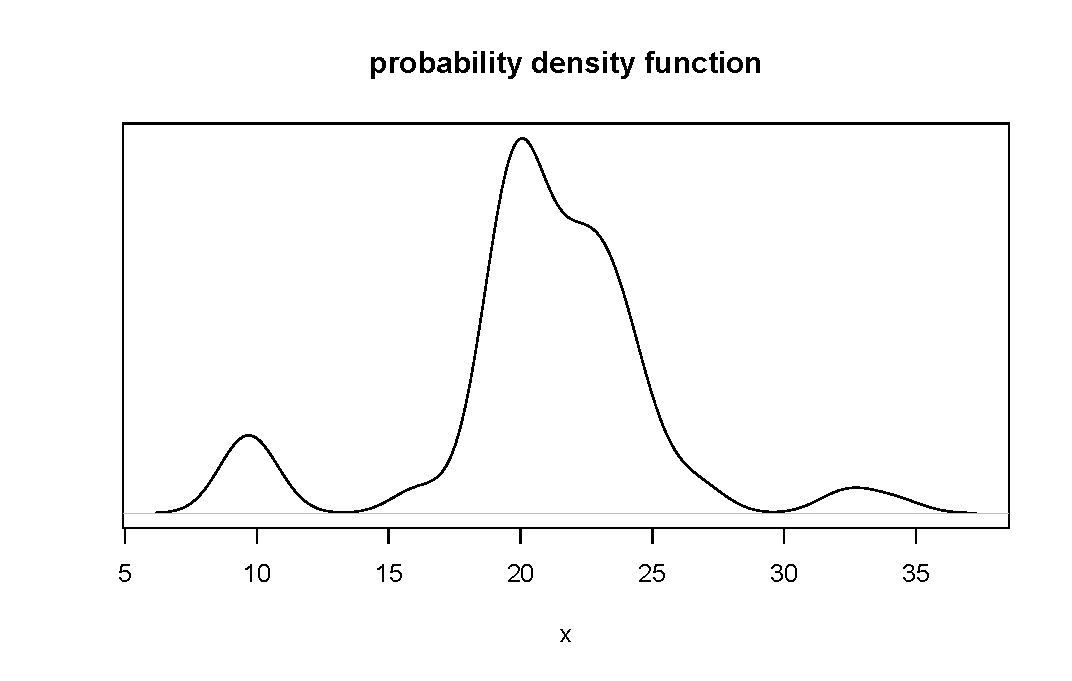
\includegraphics[width=4.25in]{../graphs/galaxy1}

The {\it marginal} density has multiple modes; one for each $\bs{\mu}_k$.

\vskip -.5cm
\end{frame}

\begin{frame}

{\bf \theme Mixture Model: \sg breaking into $\bs{K}$
  components }

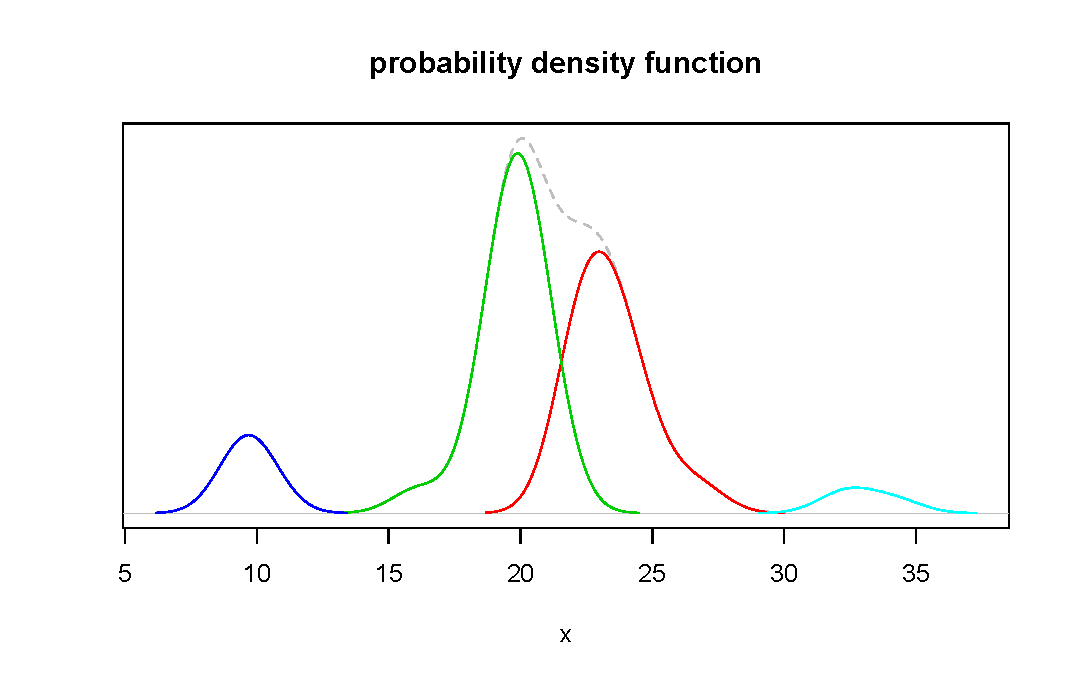
\includegraphics[width=4.25in]{../graphs/galaxy4}

Here, we have $K=4$ different cluster centers. {\gr Should it be 5?}

\vskip -.5cm
\end{frame}


\begin{frame}
{$K$-means}

$K$-means algorithm clusters data by fitting a mixture model.

\vskip .1cm
Suppose data $\bm{x}_1 \ldots \bm{x}_n$ comes from
$K$ clusters.

\vskip .1cm
If you know membership $k_i$ for each $x_i$, then estimate
\[\nv
\hat \mu_k = \frac{1}{n_k}\sum_{i:k_i=k} \bm{x}_i
\]
\hfill where $\{i:k_i=k\}$ are the $n_k$ observations in group $k$.

\sk
$K$-means finds $\bs{k} = k_1 \ldots k_n$ to minimize the
sum-of-squares
\[\nv
\sum_{k=1}\sum_{i:k_i=k} (\bm{x}_i - \bs{\hat\mu}_k)^2
\]
Mixture deviance: total sums of squares within each cluster.

\end{frame}


\begin{frame}

{\bf Give $\bs{K}$-means the $\bs{x_i}$'s, and it gives you
  back the $\bs{k_i}$'s}

\begin{columns}

\column{2.3in}

\sk
~~~~~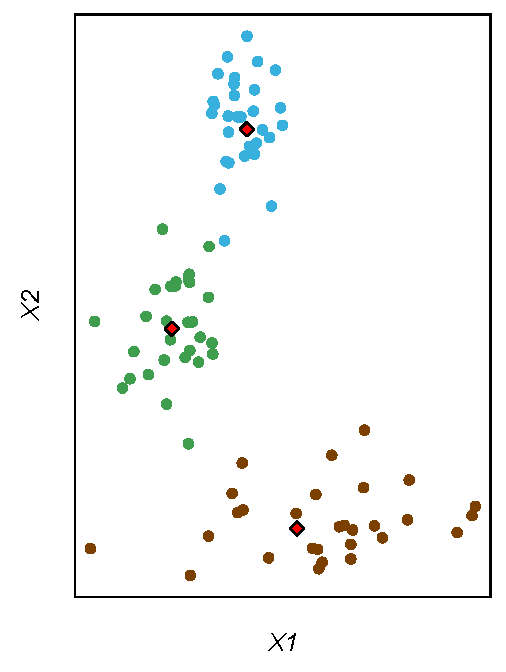
\includegraphics[width=1.8in]{../graphs/3means}

\column{3in}


This assigns a cluster to each $x_i$,\\
and implies the group means $\bs{\hat \mu}_k$.

\sk
The algorithm starts at random $\bs{k}$,\\
and changes $k_i$'s until the sum \\of squares stops improving.

\sk
 Solution depends on start location.\\
 Try
multiple,  take the best answer.
\sk
\end{columns}

\vskip .25cm
Choosing $K$: \bk
For most applications, everything is descriptive. 

So try a few and use clusters that make
sense to you.

\vskip -.5cm
\end{frame}


\begin{frame}[fragile]



{\bf kmeans(x, centers, nstart)} 


\vskip .2cm
Clusters {\tt \theme x}
{\gr (numeric!)}
into {\theme centers} groups using {\theme \tt nstart} starts.

\begin{semiverbatim}\nv \scriptsize\vspace{-.5cm}
  > grp = kmeans(x=mydata, centers=3, nstart=10)
  
  K-means clustering with 3 clusters of sizes 28, 31, 31
  Cluster means:
             x           y
  1  1.0691704 -0.99099545
  2 -0.2309448 -0.04499839
  3  0.4987361  1.01209098
  
  Clustering vector:
   [1] 2 1 1 1 1 1 1 1 1 1 3 3 3 3 3 3 3 3 3 3 2 2 2 2 2 2 2 2 2 2 
  [39] 1 1 3 3 3 3 3 3 3 3 3 3 2 2 3 2 2 2 2 2 2 2 1 1 1 1 1 1 1 1 
  
  Within cluster sum of squares by cluster:
  [1] 12.332683  4.911522  3.142067
   (between_SS / total_SS =  80.5 %)
\end{semiverbatim}
{\tt \theme grp\$cluster}
holds cluster assignments for each observation.

\end{frame}

\begin{frame}
{Scaling for $K$-means}

The algorithm minimizes total [squared] distance from center,\\
{\it summed across all dimensions of $\bm{x}$}.

\sk
Scale matters: if you replace $x_j$ with $2x_j$, that dimension \\counts twice as much in determining distance from center \\{\gr (and will have more influence on cluster membership).}

\sk
Standard solution is to standardize: 
\[\nv 
\text{cluster~on~scaled}~~\tilde x_j = \frac{x_{ij}-\bar{x}_j}{\mr{sd}(x_j)}
\]   Then the centers $\mu_{jk}$ are interpreted as\\ {\it standard deviations from marginal average}.


\end{frame}


\begin{frame}

\begin{columns}

\column{2.5in}

~~~~~~
\includegraphics[width=3in]{../graphs/frenchman}

\column{2in}

\vskip -1cm
\hskip -1cm {\bf  Clustering Europe by Food}

\sk
\hskip -1cm Protein consumption by country,\\
\hskip -1cm in grams per person per day for 

\begin{center}\gr
 Red and White Meat \\ Eggs, Milk, Fish\\     
Cereals,  Starch, Nuts \\  Fruit and Vegetables
\end{center}

\hfill See {\tt protein.R}.~~~~
\end{columns}

\end{frame}


\begin{frame}

{\bf 3-means clustering on  Red vs White meat consumption}

\vskip -.5cm
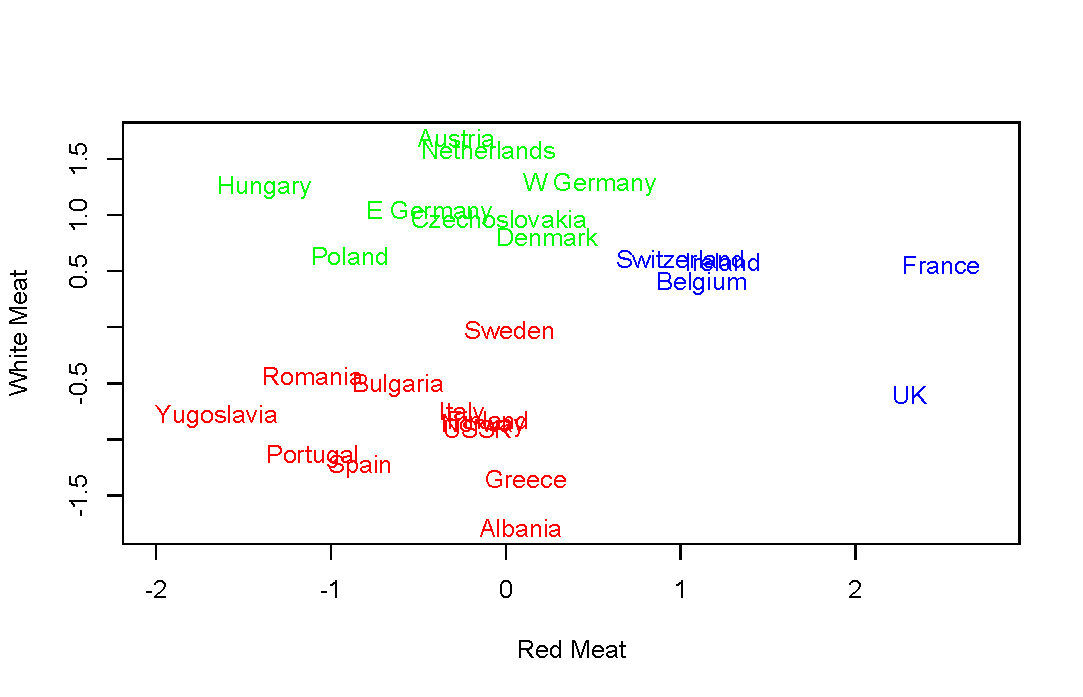
\includegraphics[width=4.25in]{FOODmeat}


Consumption is in units of standard deviation from the mean.
\end{frame}


\begin{frame}

{\bf 7-means clustering on \theme all nine protein types}

\vskip -.5cm
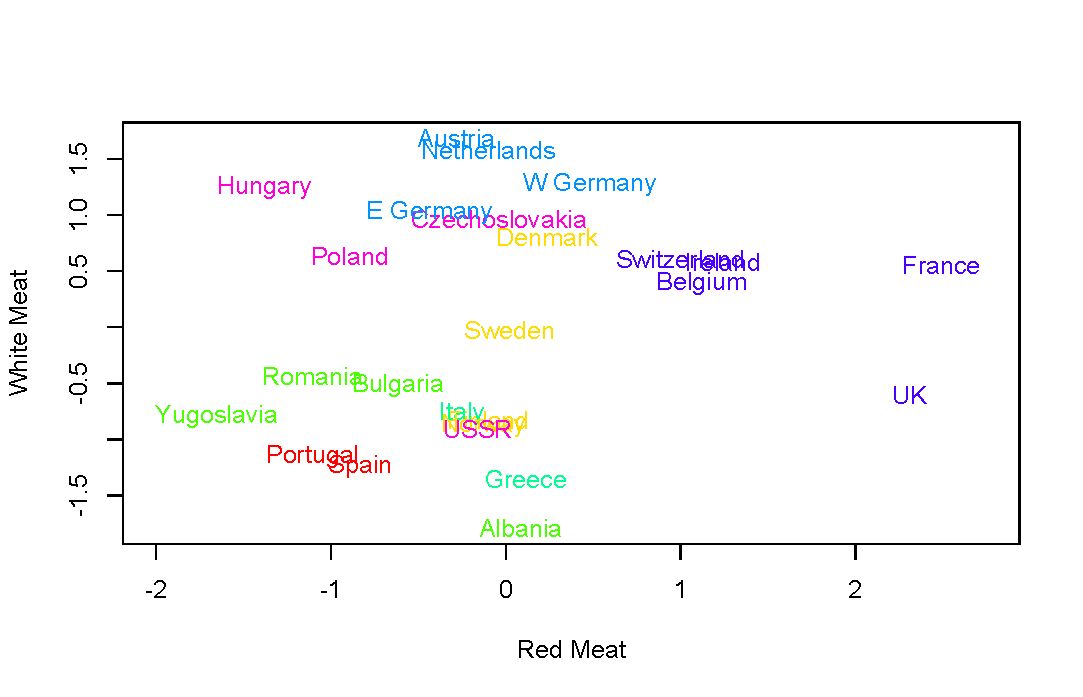
\includegraphics[width=4.25in]{FOODprotein}

Plotting the red vs white plane, but {\it clustering on all variables.}
\vskip -.5cm
\end{frame}


\begin{frame}[fragile]
{Wine Clustering}

{\gr Today is all about food!}

\vskip .25cm
{As a bigger data example, {\tt wine.csv} contains data on 11 chemical properties of {\it vino verde} wine from northern Portugal.}

\vskip .25cm
We have chemistry for 6500 bottles (1600 red, 4900 white), along with average quality rating (out of 10) by `expert' tasters.

\vskip .5cm
If you fit a 2-mean mixture, you get what you might expect
\begin{semiverbatim}\nv
> tapply(wine$color,km$cluster,table)\bk
      \$`1`           \$`2` 
        red white      red white 
         24  4830     1575    68
\end{semiverbatim}
The two clusters are red vs white wine.

\end{frame}

\begin{frame}

In 2D slices of $\bm{x}$, we see clear red v white discrimination.

\vskip .25cm
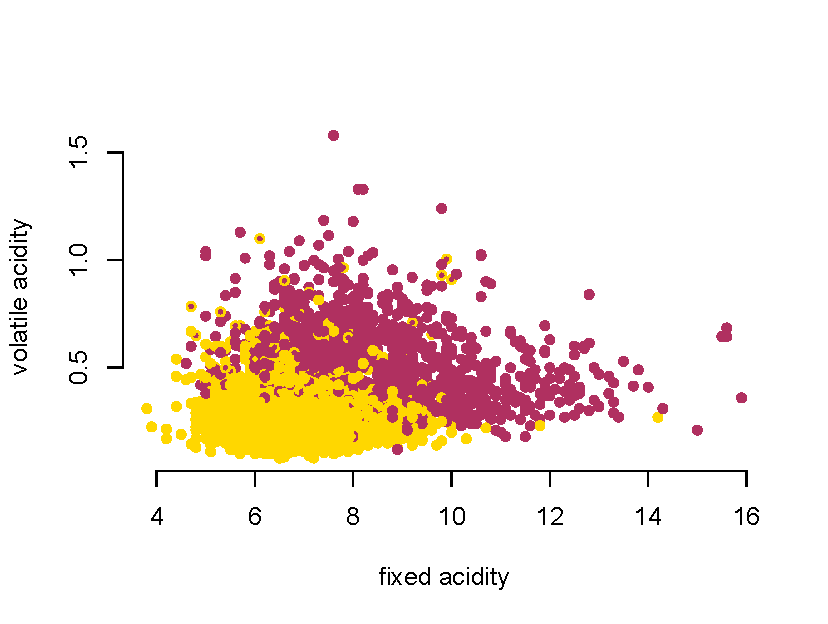
\includegraphics[width=\textwidth]{wine2D}

\gr Point border is true color, body is cluster membership.
\end{frame}

\begin{frame}
{Choosing $K$}

1st order advice: most often clustering is an exploration exercise, so choose the $K$ that makes the most sense to you.


\vskip .25cm
But, we can apply data-based model building here:
\begin{enumerate}
\item Enumerate models for $k_1 < k_2 \ldots k_K$.
\item Use a selection tool to choose the best model for new $\bm{x}$.
\end{enumerate}

\vskip .25cm
Step one is easy.  Step two is a tougher.

\vskip .25cm
For example, for CV you'd want to have high OOS $\mr{p}_{k_i}(\bm{x}_i)$. 

\vskip .1cm
But you don't know $k_i$!  {\gr This is a {\it latent} variable.}

\vskip .1cm
{There's no ground truth like $y$ to compare against.}

\end{frame}

\begin{frame}
{AIC and BIC for K-means}


We {\it can} use IC to select $K$.
\begin{itemize}
\item Deviance is (as always) D=-2logLHD, \\
which for $K$-means is the total sum of squares {\gr (slide 8)}.
\item $df$ is the number of $\mu_{kj}$: $K\times p$. {\gr (where $p$ is dimension of $\bm{x}$)}
\end{itemize}
Then our usual AICc and BIC formulas apply.

{\gr I've added these in {\tt kIC.R} your convenience.}

\vskip .5cm
{\theme Beware:} the assumptions behind both AICc and BIC calculation are only roughly true for $K$-means, and often not even that.  

\vskip .1cm
These tools are lower quality here than in regression.

\vskip .1cm
I (and others) tend to trust BIC most for mixtures.
 
\vskip .1cm
 But you're often better off just using descriptive intuition.

\end{frame}

\begin{frame}

{\bf \bl BIC \gr and \bk AICc \gr for wine $K$-means}

\vskip .1cm
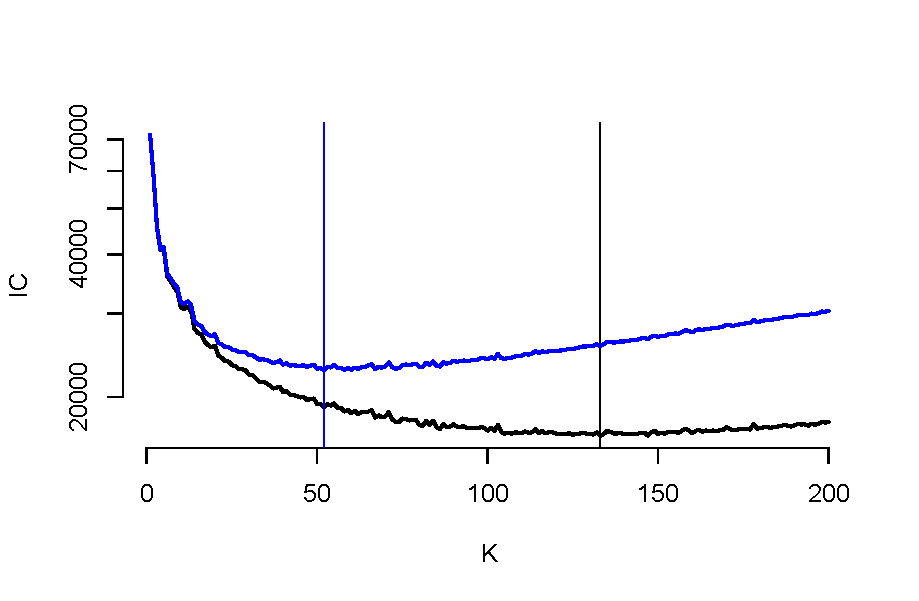
\includegraphics[width=\textwidth]{wineIC}

{BIC likes $K\approx50$, AICc likes $130$.}

Both are way more complicated than is useful.


\end{frame}


\begin{frame}[fragile]
{Cluster Regression}

\vskip .25cm
Once use of {\it unsupervised} clustering is \\ to throw the results into
a {\it supervised} regression model.

\vskip .25cm
For example, we can use the wine cluster memberships as a factor variable to predict wine quality (this is equivalent to just predicting quality with the average for each cluster).


\vskip .25cm
{\it If} the dominant sources of variation in $\bm{x}$ are related to $y$, \\this can be a good way to work.  Otherwise its not.

\vskip .25cm
The clusters all have around the same average quality
\begin{semiverbatim}\nv\small
> tapply(wine$quality,kfit[[k]]$cluster,mean)
 5.4 6.0 5.0 5.4 5.4 6.6 5.7 5.4 6.3 5.5
 6.1 5.8 5.7 6.3 6.3 6.1 5.2 6.5 5.9 5.5 
 5.3 6.1 6.2 5.4 5.1 5.9 5.5 5.9 5.5 5.3 
\end{semiverbatim}
so the strategy wouldn't work here.
\end{frame}

\begin{frame}

This isn't the same as there being no predictive power in $\bm{x}$.

\vskip .1cm
Regression onto 3-way chemistry interactions gets us\\ an OOS $R^2$ of around 33\% when predicting quality.

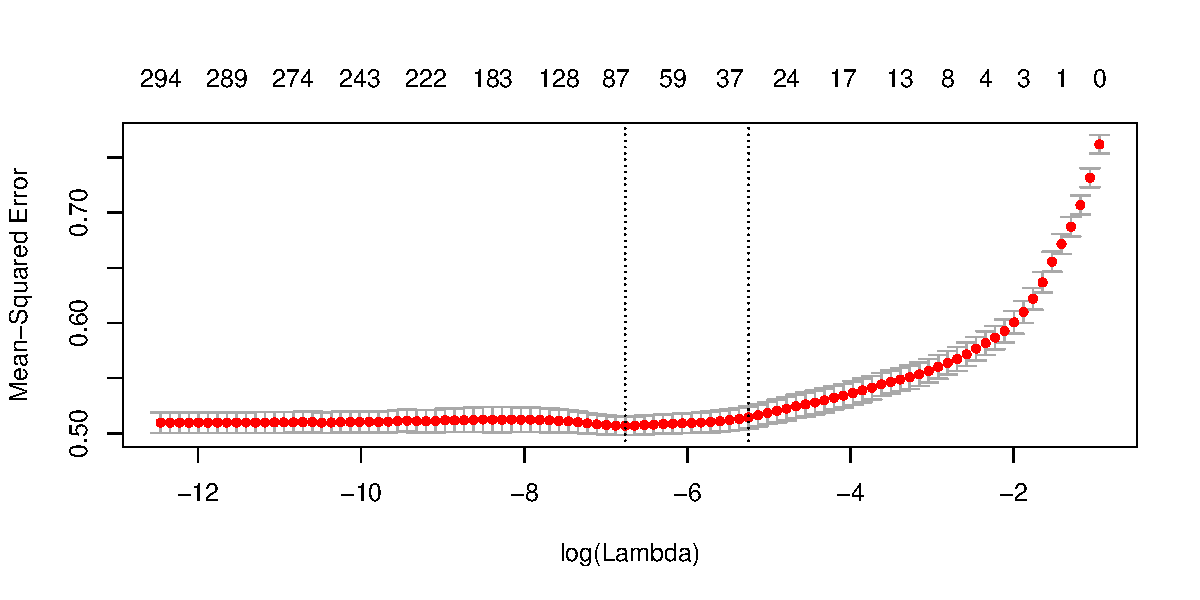
\includegraphics[width=\textwidth]{wineCV}

It's just that wine `quality' has a weak signal, and most of the variation in $\bm{x}$ is driven by other factors (e.g., grape color).

\vskip -.5cm

\end{frame}

\begin{frame}
{Re-visiting the $K$-means model}

In minimizing sums-of-squares, $K$-means targets the model
\[
\mr{p}_k(\bm{x}) = \prod_{j} \mr{N}(x_{j}\mid \mu_{kj}, \sigma^2)
\]
$\Rightarrow$ independence across dimensions {\gr (no multicollinearity)}
and uniform variance {\gr(same $\sigma$ for all $j$, which is why scale matters)}.

\vskip .25cm  Despite being a silly model, this tends to do a decent job\\ of  clustering when $\bm{x}$ consists of {\it continuous} variables.

\vskip .25cm  It does a worse job for $\bm{x}$ made up of dummies or counts.

\end{frame}

\begin{frame}
{Restaurant reviews from {\theme  we8there.com}}


\vskip .25cm 2978 bigrams from 6260 reviews (average of 90 words) with
5-star {\it overall}, {\it atmosphere}, {\it
  food}, {\it service}, and {\it value} ratings.

\sk
{\fg Great Service: 
\bk Waffle House $^\#1258$, Bossier City LA }

\vskip .2cm \sg {\footnotesize I
  normally would not revue a Waffle House but this one deserves
  it. The workers, Amanda, Amy, Cherry, James and J.D. were the most
  pleasant crew I have seen. While it was only lunch, B.L.T. and
  chili, it was great. The best thing was the 50's rock and roll
  music, not to loud not to soft. This is a rare exception to what we
  all think a Waffle House is. Keep up the good work.  

  \hfill [ 5: 5555 ]}

\sk
{\theme Terrible Service: 
\bk Sartin's Seafood, Nassau Bay TX}

\vskip .2cm\sg  {\footnotesize Had a very
  rude waitress and the manager wasn't nice either. 
 [ 1: 1115 ] }

\end{frame}

\begin{frame}
{Clustering Text}

Often, low-D structure underlies text
\begin{itemize}
\item happy/sad, document purpose, topic subject.
\end{itemize}
The $\bm{x}$ for text are {\it counts} of text {\it tokens}.

{\gr A token can be a word, bigram (pair of words), etc.}



\vskip .25cm
We can try to transform $\bm{x}$ to look like something $K$-means would work with (i.e., something that looks built out of normals).

\vskip .25cm {\tt we8there.R} fits $K$-means to standardized token proportions 
$
x_{ij}/m_i
$, where $m_i = \sum_i x_{ij}$ are the {\it document totals}.

\vskip .25cm Looking at the big $\hat\mu_{jk}$ (i.e., phrases $j$ with big
proportions in cluster $k$), it comes up with some decent interpretable factors.

\end{frame}

\begin{frame}
{Topic Models}


Although it `kinda works',  $K$-means for text is far from ideal.

Instead, use a mixture of $\mr{p}_k$ that are appropriate for count data.

\vskip .25cm
A multinomial mixture:
\begin{itemize}
\item For each word, you pick a `topic' $K$.
\item This topic has probability $\theta_{kj}$ on each word $j$.
\item You draw a random word according to $\bs{\theta}_k$
\end{itemize}

After doing this over and over for each word in your document, you've got
proportion $\omega_{i1}$ from topic 1, $\omega_{i2}$ from topic 2, etc.

\vskip .25cm
The full vector of words for document $\bm{x}_i$ then has distribution
\[\nv
\bm{x}_i \sim \text{MN}( \omega_{i1} \bs{\theta}_1 + \ldots + \omega_{iK} \bs{\theta}_K, m_i)
\]
{\it a multinomial with probabilities $\sum_k \omega_{ik}\bs{\theta}_{k}$ and total $m_i= \sum_jx_{ij}$.}

\end{frame}

\begin{frame}
{ Topic Models:  clustering for text}

Each document ($\bm{x}_i$) is drawn from a multinomial with probabilities
that are a mixture of {\theme topics} $\bs{\theta}_1\ldots\bs{\theta}_K$.
\[\nv
\bm{x}_i \sim \text{MN}( \omega_1 \bs{\theta}_1 + \ldots + \omega_K \bs{\theta}_K, m)
\]
These $\bs{\theta}$'s are topics of phrase-probabilities: $\sum_{j=1}^p
\theta_{kj} =1$.\\

e.g., a {\theme  hotdog} topic has high probability on {\theme 
  mustard, relish, ...}.

\sk
The doc weights $\bs{\omega}_i$ are also probabilities: $\sum_{k=1}^K
\omega_{ik} =1$.\\{\gr
e.g., a hotdog stand review has big $\omega_{ki}$ on the hotdog topic.}

\sk
This is subtly different from $K$-means: instead of each {\it document} $i$ being from a cluster, now each {\it word} is from a different topic and the document is a mixture of topics.

\end{frame}

\begin{frame}[fragile]
{Fitting topic models in R}


{\tt maptpx} package has a {\tt topics} function; see {\tt ?topics}.
\begin{semiverbatim}\nv
tpc <- topics(x,K=10,tol=10)\gr # 10 topic model
\end{semiverbatim}

Fitting a topic model is computationally very difficult.

\vskip .1cm
Just like in $K$-means, 
we need only roughly estimate $\bs{\hat \theta}_k$ (analogous to $\bm{\mu}_k$) to get a decent clustering.
\vskip .1cm
So Big Data implementations use approximate (stochastic) deviance minimization.

\sk
{\gr Plenty of other packages out there; note that 
topic modeling is also called LDA (latent Dirichlet allocation) if you're exploring.}

\end{frame}



\begin{frame}[fragile]
{Selecting the number of topics}


{Choosing $K$ here is same as in $K$-means: this is exploratory analysis, so 
just choose what you want for story-telling.}

\vskip .25cm
But, you can use BIC: if you give ${\tt topics}$ a vector for {\tt K}, it incrementally grows  and stops when the BIC keeps increasing.

It reports {\tt log Bayes Factor}, which is like {\tt -BIC}.

\vskip .25cm
The model returned is that for $K$ with lowest BIC (highest BF).

\begin{semiverbatim}\footnotesize\nv
        Log Bayes factor and estimated dispersion:
                     5       10      15        20
        logBF 76020.73 90041.99 7651.02 -62745.37
        Disp      7.19     5.06    4.02      3.43
\end{semiverbatim}
Here, max BF selects $K=10$ {\gr (don't worry about `dispersion')}.
\end{frame}

\begin{frame}[fragile]
{Interpreting topics}

{We build interpretation by looking at `top' words for each topic.}

\vskip .1cm
 You can order by lift: $\theta_{jk}/${\tt mean(X[,j]/m)}.

\begin{semiverbatim}\nv\scriptsize\vspace{-.25cm}
summary(tpcs)\bk
Top 5 phrases by topic-over-null term lift (and usage \%):
[1] food great, great food, veri good, food veri, veri nice (13.7) 
[2] over minut, ask manag, flag down, speak manag, arriv after (11.6) 
\end{semiverbatim}

\vskip .1cm
Sometimes straight word probabilities are more intuitive

\begin{semiverbatim}\nv\scriptsize\vspace{-.25cm}
rownames(tpcs$theta)[order(tpcs$theta[,1], decreasing=TRUE)[1:10]]\bk
  veri good great food food great great place veri nice   
  wait staff   good food    food excel   great servic place eat \nv
rownames(tpcs$theta)[order(tpcs$theta[,2], decreasing=TRUE)[1:10]]\bk
  go back came out tast like never go brought out
  wait minut  take order  minut later come out    drink order
\end{semiverbatim}


Here, topic 1 looks `good' and 2 looks `bad'.

\end{frame}


\begin{frame}[fragile]

{\bf \gr Wordles!}

\vskip .25cm

You can use the {\tt wordcloud} library to efficiently visualize.

{\footnotesize
\verb!wordcloud(row.names(theta), freq=theta[,2], min.freq=0.004)!}

\vskip .25cm
{\gr ~~~~~~~~~~Topic 1 ~~~~~~~~~~~~~~~~~~~~~~~~~~~~ Topic 2}
~~~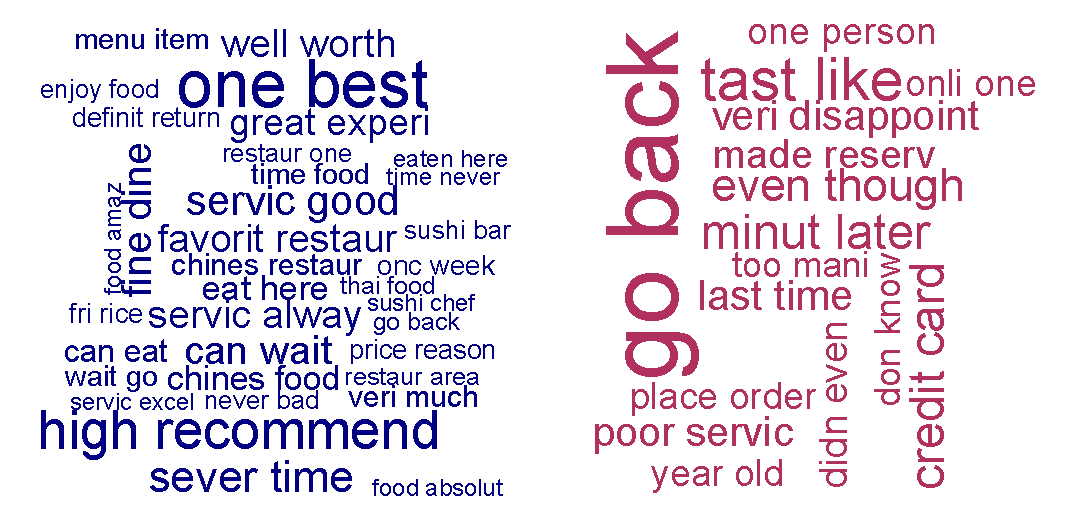
\includegraphics[width=4in]{../graphs/we8wordle}

\vskip .1cm
{\gr In the language of wordles, {\tt freq} controls word size.  \\I've made word size proportional to the in-topic probability.}

\end{frame}

\begin{frame}[fragile]{Topic Regression}

{Just like with $K$-means, we can relate topics to other \\variables in a second-stage low-D regression.}

\vskip .25cm

Here, the topics looked motivated by quality. 

Perhaps they'll be useful in predicting review rating?

\begin{semiverbatim}\nv\footnotesize
stars <- we8thereRatings[,"Overall"]
tpcreg <- gamlr(tpcs\$omega, stars)
\gr# Effect stars from 10\% increase in topic use\bk
drop(coef(tpcreg))*0.1 
     intercept      1      2      3      4   
         0.414  0.075 -0.386  0.068  0.042   
             5      6     7     8      9     10 
         0.000  0.076 0.121 0.000 -0.134 -0.049 
\end{semiverbatim}
So, e.g., you drop an expected -.4 star for if an extra 10\% of the review comes from topic 2 here (our negative topic from above).

\end{frame}

\begin{frame}

Comparison regressing {\tt stars} on bigram proportions $x_{ij}/m_i$.

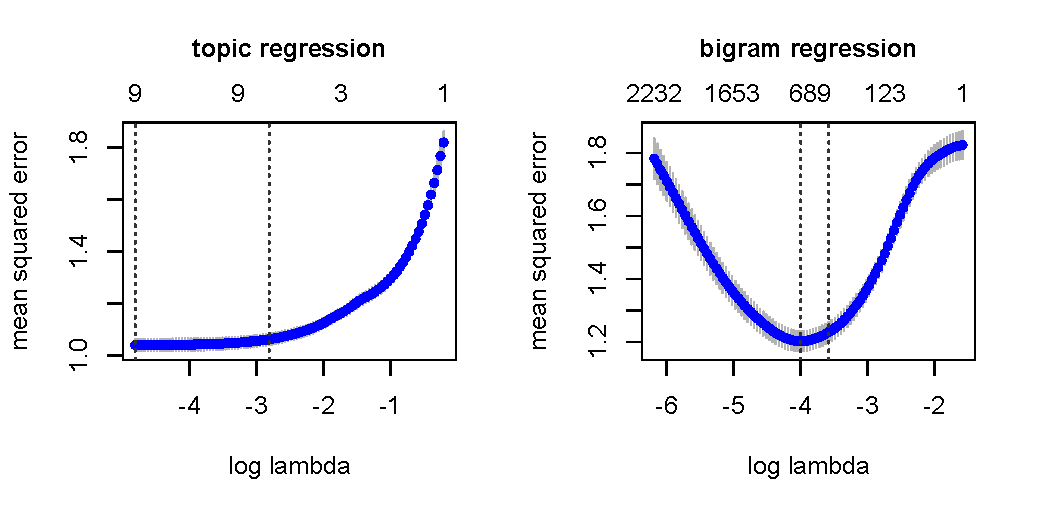
\includegraphics[width=\textwidth]{we8thereCV}

The topic model does better than regression onto words!
\end{frame}

\begin{frame}
{Round up on unsupervised clustering}


It is largely an exploratory analysis technique.  

\vskip .1cm
Don't be too fancy in your rules to choose $K$, because all that matters is that the model tells an intuitive story.

\sk
You can use clustering results as inputs for low-D regressions.  

\vskip .2cm
This is great if the dominant sources of variation in $\bm{x}$ are \\related to $y$ 
{\gr (especially if you have more $\bm{x}_i$'s than $y_i$'s).}

\vskip .2cm
But it's useless if $y$ is not connected main drivers behind $x$, \\ 
\hfill as is common in big data!~~~

\end{frame}

\begin{frame}
{Computational Roundup}

Both $K$ and topic modeling take a long time:\\
\hfill clustering uses massively high dimensional models ($K\times p$)

\vskip .25cm
There are approximate distributed algorithms \\
{\gr (e.g., stochastic descent)}.

\vskip .25cm
For really big data, just fit on subsamples:  \\since unsupervised clustering is driven by dominant\\ sources of variation, you shouldn't need all the data.


\end{frame}

\begin{frame}
{Speech in the 109th Congress}

{\tt textir} contains {\tt congress109} data: counts for 1k phrases
used by each of 529 members of the 109th US congress.

{\gr Load it with {\tt data(congress109)}.  See {\tt ?congress109}.}

\vskip .2cm
The counts are in {\tt congress109Counts}.  

\vskip .1cm
We also have {\tt congress109Ideology},
a data.frame containing some information about each speaker.

\vskip .1cm
The includes some partisan metrics:
\begin{itemize}
\item party (‘R’epublican, ‘D’emocrat, or ‘I’ndependent)
\item {\tt repshare}: share of constituents voting for Bush in 2004.
\item Common Scores [cs1,cs2]: basically, the first two principal components of roll-call votes (next week!).
\end{itemize}


\end{frame}

\begin{frame}
{Homework due next week: congressional speech}

[1] Fit $K$-means to speech text for $K$ in 5,10,15,20,25.  \\Use BIC to choose the
 $K$ and interpret the selected model.

\vskip .25cm
[2] Fit  a topic model for the speech counts.  Use Bayes factors to choose the number of topics, and interpret your chosen model.

\vskip .25cm
[3] Connect the unsupervised clusters to partisanship.
\begin{itemize}
\item tabulate party membership by $K$-means cluster.  \\Are there any non-partisan topics?
\item fit topic regressions for each of {\tt party} and {\tt repshare}.  Compare to regression onto phrase percentages:
\end{itemize}
{\tt \nv\small x<-100*congress109Counts/rowSums(congress109Counts) }

\vskip .2cm
{\gr No starter scipt; look at {\tt we8there.R} and {\tt wine.R}.}

\end{frame}

\end{document}
